
% \section{Vorticity and Potential Vorticity}
\begin{frame}{What is Vorticity?}
    \begin{columns}
      \column{0.6\textwidth}
      \begin{itemize}
        \item \textbf{Vorticity} quantifies the local rotation in a fluid flow.
        \item Defined as the \textbf{curl} of the velocity field:
        \[
          \vec{\zeta} = \nabla \times \vec{u}
        \]
        \item For 2D flow \( \vec{u} = (u(x,y), v(x,y)) \), only the \(z\)-component matters:
        \[
          \zeta = \frac{\partial v}{\partial x} - \frac{\partial u}{\partial y}
        \]
        \item \(\zeta > 0\): Cyclonic (counter-clockwise) rotation
        \item \(\zeta < 0\): Anticyclonic (clockwise) rotation
      \end{itemize}
    
      \column{0.4\textwidth}
      \vspace{2cm}  % Optional vertical spacing to balance columns
    \end{columns}
    \end{frame}
    

\begin{frame}{Zero Vorticity (Uniform Flow)}
    \begin{columns}
      \column{0.5\textwidth}
      \begin{itemize}
        \item \( \vec{u} = (2, 0) \)
        \item Uniform horizontal flow
        \item No shear or curvature
        \item \( \zeta = 0 \)
      \end{itemize}
    
      \column{0.5\textwidth}
      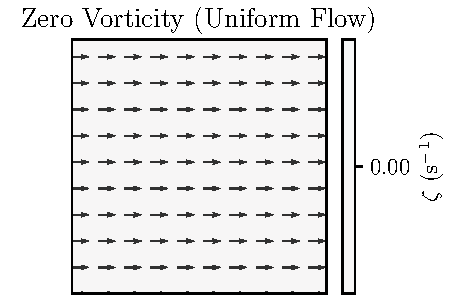
\includegraphics[width=\linewidth]{../images/vorticity_plot0.pdf}
    \end{columns}
    \end{frame}
    
    \begin{frame}{Shear Vorticity}
    \begin{columns}
      \column{0.5\textwidth}
      \begin{itemize}
        \item \( \vec{u} = (y, 0) \)
        \item Horizontal shear: \( \frac{\partial u}{\partial y} = 1 \)
        \item \( \zeta = -1 \)
      \end{itemize}
    
      \column{0.5\textwidth}
      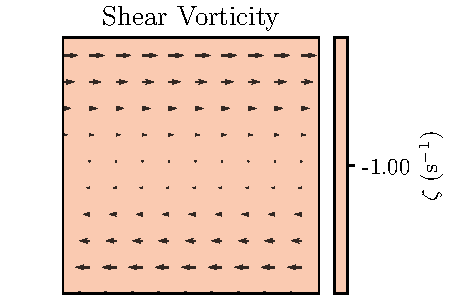
\includegraphics[width=\linewidth]{../images/vorticity_plot1.pdf}
    \end{columns}
    \end{frame}
    
    \begin{frame}{Nonlinear Shear Vorticity}
    \begin{columns}
      \column{0.5\textwidth}
      \begin{itemize}
        \item \( \vec{u} = (y^2, 0) \)
        \item \( \zeta = -2y \)
        \item Antisymmetric vorticity field
        \item Stronger at larger \( |y| \)
      \end{itemize}
    
      \column{0.5\textwidth}
      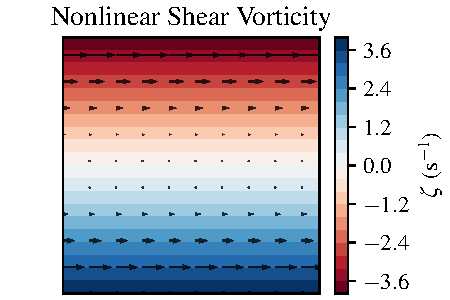
\includegraphics[width=\linewidth]{../images/vorticity_plot2.pdf}
    \end{columns}
    \end{frame}
    
    \begin{frame}{Positive Vorticity (Cyclonic)}
    \begin{columns}
      \column{0.5\textwidth}
      \begin{itemize}
        \item \( \vec{u} = (-y, x) \)
        \item Pure rotation, counter-clockwise
        \item \( \zeta = 2 \)
      \end{itemize}
    
      \column{0.5\textwidth}
      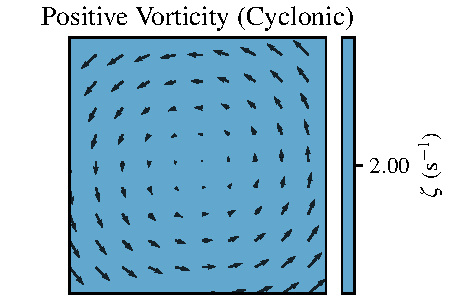
\includegraphics[width=\linewidth]{../images/vorticity_plot3.pdf}
    \end{columns}
    \end{frame}
    
    \begin{frame}{Negative Vorticity (Anticyclonic)}
    \begin{columns}
      \column{0.5\textwidth}
      \begin{itemize}
        \item \( \vec{u} = (y, -x) \)
        \item Clockwise rotation
        \item \( \zeta = -2 \)
      \end{itemize}
    
      \column{0.5\textwidth}
      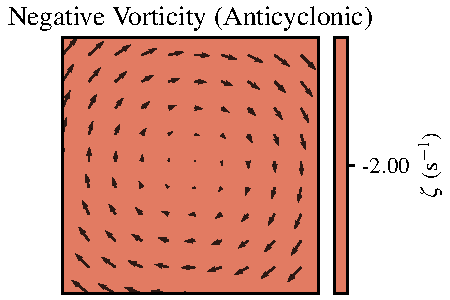
\includegraphics[width=\linewidth]{../images/vorticity_plot4.pdf}
    \end{columns}
    \end{frame}

    \begin{frame}{Absolute Vorticity}
        \begin{columns}
          \column{0.6\textwidth}
          \begin{itemize}
            \item In a rotating frame (like Earth), the total or \textbf{absolute vorticity} is:
            \[
              \eta = f + \zeta
            \]
            \item \( \zeta \): relative vorticity (from local shear and curvature)
            \item \( f = 2\Omega \sin\phi \): Coriolis parameter, varies with latitude
            \item Important for large-scale geophysical flows (e.g., Rossby waves, PV conservation)
          \end{itemize}
        
          \column{0.4\textwidth}
          \vspace{2cm}
        \end{columns}
        \end{frame}
        
        \begin{frame}{Konservierung der potentiellen Vorticity}
            \begin{columns}
              \column{0.6\textwidth}
              \begin{itemize}
                \item Die \textbf{potentielle Vorticity (PV)} ist gegeben durch:
                \[
                  q = \frac{\eta}{H} = \frac{f + \zeta}{H}
                \]
                \item \( \eta \): absolute Vorticity, \( f + \zeta \)
                \item \( H \): effektive Schichtdicke (z.B. Troposphärenhöhe oder isentrope Schichtdicke)
                \item In der reibungsfreien, adiabatischen Atmosphäre gilt:
                \[
                  \frac{Dq}{Dt} = 0
                \]
                \item \textbf{Implikation:} PV ist entlang von Teilchenbahnen erhalten → zentrale Rolle in der großräumigen Dynamik
              \end{itemize}
            
              \column{0.4\textwidth}
              \vspace{2cm}
            \end{columns}
            \end{frame}
            

            \begin{frame}{Barotrope Vorticity-Gleichung}
                \begin{itemize}
                  \item Annahmen:
                  \begin{itemize}
                    \item Nicht-divergente Strömung
                    \item Eine Schicht (barotropes Modell)
                  \end{itemize}
                  \item Vorticity-Gleichung (mit \(\psi\): Stromfunktion):
                  \[
                    \frac{\partial}{\partial t}(\nabla^2 \psi) + \beta \frac{\partial \psi}{\partial x} = 0
                  \]
                  \item Wellenlösung: 
                  \[
                    \psi = \Re \left\{ \hat{\psi} \, e^{i(kx + ly - \omega t)} \right\}
                  \]
                  \item Dispersionsrelation:
                  \[
                    \omega = -\beta \frac{k}{k^2 + l^2}
                  \]
                  \item \textbf{Folgen}:
                  \begin{itemize}
                    \item Westwärts laufende Rossby-Wellen (\( \omega < 0 \) für \( k > 0 \))
                    \item Phasengeschwindigkeit \( \neq \) Gruppengeschwindigkeit
                  \end{itemize}
                \end{itemize}
                \end{frame}
                